% format: latex
%%--------------------------------------------------------------------------
%%  This is a sample LaTeX2e input file for the University of Pittsburgh
%%  thesis document class (pitthesis.cls).
%%
%%  Wonkoo Kim (wkim+@pitt.edu, wkim@bellatlantic.net), September 23, 1999
%%--------------------------------------------------------------------------
%%
%%  A '%' character causes TeX to ignore all remaining text on the line,
%%  and is used for comments like this line.
%%

%\documentclass [12pt,proposal]{pitthesis}
%\documentclass [12pt]{pitthesis}
\documentclass [10pt]{pitthesis}
%\documentclass [12pt,twoside]{pitthesis}

%%
%%  Pitt Thesis Document Class:
%%
%%	This document class loads latex2e's report class.
%%	A latex2e thesis document starts with
%%
%%	\documentclass[options]{pitthesis}
%%
%%	Additional class options to the report class are provided for
%%	Pitt thesis styles.
%%
%%  Pitt Thesis Document Class Options:
%%
%%	pitteng     Pitt Engineering thesis (selected by default)
%%	pittstd     Pitt (Standard) thesis (selects nofloatchap by default)
%%	phd	    Ph.D thesis (selected by default)
%%	ms	    M.S. thesis
%%	proposal    for proposal presentation
%%	headings    default running heads with page numbers
%%	noheadings  do not put default running heads
%%	floatchap   floats (figures and tables) are numbered by chapters
%%	nofloatchap floats (figures and tables) are numbered sequentially
%%	single	    single line spacing
%%	onehalf     one and half (1.5) line spacing (selected by default)
%%	double	    double line spacing
%%
%%	(And, all `report' class options can be used.)
%%
%%  Default Options:	11pt, pitteng, phd, noheadings, onehalf
%%			floatchap   -- for pitteng
%%			nofloatchap -- for pittstd
%%
%%  If no options were given for pitthesis class, then
%%  [11pt,pitteng,phd,noheading,onehalf] are selected by default.
%%  For example, a typical 12pt Pitt Engineering Ph.D thesis document will
%%  start with
%%	\documentclass[12pt]{pitthesis}
%%  or, \documentclass[12pt,pitteng,phd]{pitthesis}
%%
%% Numbering Floats (Figures and Tables):
%%
%%  For Engineering thesis, floats(figures,tables) are numbered by
%%  chapters and appendices if `nofloatchap' class option was not given.
%%  When `nofloatchap' option is chosen, all figures and tables are numbered
%%  sequentially throughtout the whole document including appendices.  If you
%%  want to number figures and tables in appendices separately, then the
%%  command \floatsbyappendix can be used anywhere before appendix in a
%%  document.  Then figures and tables in appendices are numbered like A-1,
%%  A-2, B-1, etc.
%%
%%  \documentclass[nofloatchap]{pitthesis}
%%			-- floats(figures,tables) are numbered sequentially
%%			   throughout the whole document.
%%
%%  \floatsbyappendix	-- floats(figures,tables) are numbered by appendices
%%			   if this command is used in a user document.

% The preamble begins here.

%\floatsbyappendix

\usepackage{graphicx}
\newif\ifAMS
\IfFileExists{amsfonts.sty}
  {\AMStrue\usepackage{amsmath,amsthm,amsfonts}}
  {\usepackage{latexsym}}


% Declares the document's title.
\title{ USING \LaTeX\ TO WRITE A PITT THESIS
--- A Sample Document File}

%\proposal{Ph.D. Dissertation Proposal} % print on title page by 'proposal' option

\author{Wonkoo Kim}			% Declares the author's name.

% Declares formerly earned degrees
\degrees{B.S. in E.E., Sogang University, Korea, 1979\\
M.S. in E.E., Korea Advanced Institute of Science and Technology, 1982}

% Declares degree to earn
\degree{Doctor\\of\\Philosophy}
%\degree{Master of Science\\in\\Electrical Engineering} % for M.S.

\school{School of Engineering}		% for School of Engineering thesis
%\school{School of Arts and Science}	% for other Pitt schools
\university{University of Pittsburgh}	% the University

\date{September 23, 1999}   % Deleting this command produces today's date.

\year{1999}		% year in title page

%\renewcommand{\baselinestretch}{1.3}	% line spacing

%%---------------------------------------------------------------------------
\begin{document}
%%---------------------------------------------------------------------------

\maketitle		% Produces the title.

\begin{committeesignature}[5]	% begin the committee the signature page.
% It has an optional argument for the number of committee members.
% If you have more or less than 5 committee members, give the number in the
% optional argument for better spacing between signature fields.
% e.g., \begin{committeesignature}[4] for 4 committee members including advisor.

%% Committee members in {committeesignature} environment must be placed with
%% proper ordering, as those members will be typeset immediately at the
%% commands.
%% \chairperson{} is the synonym of \advisor{}.
%% \cochairperson is the synonym of \coadvisor{}.
%% Use \committeemember{} for additional committee members

%% For Ph.D. Thesis
\advisor{Firstname1 Lastname1, Ph.D. (Electrical Engneering)}
			% \chairperson is a synonym of \advisor{}
%\coadvisor{Prof. Foo Bar, Ph.D.}   % if you have a Co-advisor
			% \cochairperson is a synonym of \coadvisor{}
\committeemember{Firstname2 Lastname2, Ph.D. (Electrical Engineering)}
\committeemember{Firstname3 Lastname3, Ph.D. (Electrical Engineering)}
\committeemember{Firstname4 Lastname4, Ph.D. (Mathematics)}
\committeemember{Firstname5 Lastname5, Ph.D. (Electrical Engineering)}

\end{committeesignature}	% end the committee signature page.

%% For M.S. Thesis
%    \begin{committeesignature}
%    \advisor{Prof. Foo Bar, Ph.D.}
%    \end{committeesignature}

\chapter*{ACKNOWLEDGMENTS}

Write your acknowledgment texts here.



\advisorname{Firstname1 Lastname1, Ph.D.}   % for PhD thesis abstract page
\abstract		% generate the heading of abstract page
%%% abstract
%%% ---------------------------------------------------------------------------
\begingroup

%%% english
%%% ...........................................................................
\addchap{Abstract}

\blindtext


%%% german
%%% ...........................................................................
\otherlanguage{ngerman}
\addchap{Kurzfassung}

\blindtext

\endgroup

\tableofcontents

\listoffigures

\listoftables

% master: main
% format: latex

%%--------------------------------------------------------------------------
\chapter*{NOMENCLATURE}
%%--------------------------------------------------------------------------

\begin{list} {} {\labelwidth 6em \leftmargin 8em \labelsep 1.5em}

\item[$:=$] denotes definition.

\item[$\left\lfloor \cdot \right\rfloor$] The largest integer less than
	$\cdot$.

\item[$H(z)$] The Z-transform of a coefficient sequence $h[n]$ is
    defined by
    $$
	H(z) := \sum_{n=-\infty}^\infty h[n] z^{-n}.
    $$

\item[$\rho(\mathbf{A})$] The spectral radius of a matrix $\mathbf{A}$ is defined
    by
    \[
	\rho(\mathbf{A}) := \limsup_{m\rightarrow\infty} \left\|\mathbf{A}^m\right\|^{1/m}.
    \]

\item[$\sigma(\mathbf{A})$] The largest eigenvalue of a matrix $\mathbf{A}$ is
	defined by
    \[
	\sigma(\mathbf{A}) := \max\{\:\left|\lambda\right|\::\: \mbox{$\lambda$ is an
				eigenvalue of $\mathbf{A}$}\}.
    \]
    Note that $\rho(\mathbf{A}) = \sigma(\mathbf{A}).$

\end{list}

%%--------------------------------------------------------------------------
\section*{ABBREVIATIONS}
%%--------------------------------------------------------------------------

\begin{list} {} {\labelwidth 6em \leftmargin 8em \labelsep 1.5em}

\item[AMS]  American Mathematical Society
\item[CTAN] Comprehensive \TeX\ Archive Network, e.g., \\
	\verb|http://ctan.tug.org|, 
	\verb|ftp://ctan.tug.org/tex-archive|

\end{list}
	% nomenclature and abbreviations

%%--------------------------------------------------------------------------
%\pagenumbering{arabic}
% master: main
% format: latex

%%--------------------------------------------------------------------------
\part{\LaTeXe\ Document Class for Pitt Theses}
%%--------------------------------------------------------------------------

This document will illustrate some of the \LaTeX\ powers in typesetting
a thesis at University of Pittsburgh. The source file of this document
will be used as a sample \LaTeXe\ file for thesis writing.
It is to be compiled with \LaTeXe, and the following class files should be
accessible for writing thesis at University of Pittsburgh during the
compilation: \\

\begin{tabular}{ll}
\texttt{pitthesis.cls} & the main Pitt thesis document class file \\
\texttt{pitteng.clo}   & class option file for Pitt Engineering thesis \\
\texttt{pittstd.clo}   & class option file for Pitt standard thesis \\
\end{tabular} \\

The document is divided into three parts. The first part describes the usage of
the document class \texttt{pitthesis}.	The second part is the level one sample
input.	Except some sectioning headings added in by the current author for
illustration and clarity, it is the verbatim copy of the Leslie~Lamport's
\texttt{sample2e.tex} (which is a sample file from the \LaTeXe\ package).
Effort is made for the user to see most of the likely needed \LaTeXe\ commands
in writing a thesis.  The User should compare this source file with the
document result as well as the \LaTeXe\ Manual.\cite{lp:latex}
The third part is for the mathematical equations (instead of simple formula)
and figures/tables and the third part is about the special symbols.
I recommend the user compare every command used in this file with the document
result and the \LaTeXe\ Manual, but some of the commands may not be found there,
in AMS\LaTeX\ by the American Mathematical Society, which can be obtained from
CTAN (Comprehensive TeX Archive Network) sites, e.g.,
\verb|ftp://ctan.tug.org/tex-archive/macros/latex/|.
The bibliography is also sneaked in. The user should also watch out for it.

%%--------------------------------------------------------------------------
\chapter{PITT THESIS DOCUMENT CLASS OPTIONS}
%%--------------------------------------------------------------------------

Pitt thesis document class package (including this document) borrowed some
Jinbai Wang's work on \LaTeX 2.09 style files for theses at the University of
Pittsburgh\cite{jbw:tex} and is completely rewritten by the current author
for \LaTeXe 's report class, so that all options of report class can be used.
The reader should also notice that the document class \textbf{pittthesis} that
I wrote has two important class options, \texttt{pitteng} and \texttt{pittstd},
namely, \textbf{engineering thesis} (by default) and \textbf{Pitt standard
thesis}, respectively.	One has to give the option ``\texttt{pittstd}'' for
Pitt standard thesis style, otherwise ``\texttt{pitteng}'' is assumed.
\begin{verbatim}
\documentclass{pitthesis}	    % document class for Engineering thesis.
\documentclass[pittstd]{pitthesis}  % for Pitt standard thesis.
\end{verbatim}
These classes are designed so close as possible to the thesis requirements set
by various schools at the University of Pittsburgh (including the School of
Engineering)\cite{pitteng:thesis,pittstd:thesis}. However, minor modifications
may have to be done by the individual users to fit individual needs.
A \LaTeXe\ document for a Pitt thesis starts with
\begin{verbatim}
\documentclass[options]{pitthesis}
\end{verbatim}
Note that any report class options may be used and additional class options are
provided by the \texttt{pitthesis} class for theses at the University of
Pittsburgh, which are listed in Table \ref{tab:pitthesis}.
%
\begin{table}[b!]
  \centering
  \caption{\{\texttt{pitthesis}\} document class options}
  \label{tab:pitthesis}
  \begin{tabular}{ll}
    \hline
    \verb|pitteng|*   & Pitt Engineering thesis \\
    \verb|pittstd|  & Pitt (Standard) thesis
			(selects \texttt{nofloatchap} by default)\\
    \verb|phd|*       & Ph.D. thesis \\
    \verb|ms|	      & M.S. thesis \\
    \verb|proposal|   & for proposal presentation \\
    \verb|headings|   & default running heads with page numbers \\
    \verb|noheadings|* & do not put default running heads \\
    \verb|floatchap|* & floats (figures and tables) are numbered by chapters \\
    \verb|nofloatchap|& floats (figures and tables) are numbered sequentially\\
    \verb|single|	& single line spacing \\
    \verb|onehalf|*	& 1.5 line spacing \\
    \verb|double|	& double line spacing \\
    \hline
  \end{tabular} \\
  (* are the default options.)
\end{table}
%
The default options are \texttt{11pt}, \texttt{pitteng}, \texttt{phd},
\texttt{noheadings}, \texttt{onehalf}.	And, \texttt{floatchap} is selected
by default for \texttt{pitteng} and \texttt{nofloatchap} for \texttt{pittstd},
respectively.
Hence,
\begin{verbatim}
 \documentclass{pitthesis}
\end{verbatim}
is equivalent to
\begin{verbatim}
 \documentclass[11pt,pitteng,phd,noheadings,onehalf,floatchap]{pitthesis}
\end{verbatim}
and
\begin{verbatim}
 \documentclass[pittstd]{pitthesis}
\end{verbatim}
is equivalent to
\begin{verbatim}
 \documentclass[11pt,pittstd,phd,noheadings,onehalf,nofloatchap]{pitthesis}
\end{verbatim}
For Engineering thesis, floats (figures,tables) will be numbered by
chapters and appendices if the class option \texttt{nofloatchap} is not given.
If the option \texttt{nofloatchap} is given, all figures and tables will be
numbered sequentially throughtout the whole document including appendices.
If you want to number figures and tables separately for appendices, then the
command \verb|\floatsbyappendix| can be used anywhere before appendix
environment in the document. Then figures and tables in appendices are numbered
like A-1, A-2, B-1, etc.
A typical 12pt Pitt Engineering Ph.D. thesis document may start with
\begin{verbatim}
 \documentclass[12pt]{pitthesis}
\end{verbatim}
For double-sided printing, which would be handy for personal copies,
\begin{verbatim}
 \documentclass[12pt,twoside]{pitthesis}
\end{verbatim}
will typeset even and odd pages differently with proper margins for binding
and the page numbers are printed away from the bound sides of papers.
The \texttt{twoside} option may not change the page numbers unless
a \verb|\part{}| sectioning command is used in a thesis.

\section{Line Spacing}
The line spacing of texts can be selected by the class options of
\texttt{single}, \texttt{onehalf}, and \texttt{double}.  The default line
spacing is \texttt{onehalf} (1.5 line spacing), which I prefer for the final
printout, but double line spaced texts will give more space for proofreading.
A double line spaced thesis can be created by
\begin{verbatim}
 \documentclass[12pt,double]{pitthesis}
\end{verbatim}
The line spacing of texts can be further controlled by using
\verb|\baselinestretch| in the preamble of your document.  For example,
\begin{verbatim}
 \renewcommand{\baselinestretch}{1.3}
\end{verbatim}
will stretch the line spacing of texts.  As \verb|\baselineskip| is set
right after \verb|\begin{document}| by \texttt{pitthesis} class,
\verb|\baselinestretch| does not change the line spacing of the main texts
but the line spacing of other texts like tables.

%%--------------------------------------------------------------------------
\chapter{USING \texttt{pittthesis} DOCUMENT CLASS}
%%--------------------------------------------------------------------------

\section{Thesis Title Page}
Thesis title page carries much more information than the original \LaTeXe 's
\verb|\maketitle| can handle.  Therefore, more fields are introduced to
\verb|\maketitle| for the thesis classes (Please look at the source file
(\texttt{part1.tex}) of this document).  Beside the standard fields, i.e.
\verb|\title{}|, \verb|\author{}|, and \verb|\date{}|, the following additional
fields are introduced (these can not be found in the \LaTeXe\ manual).
\begin{enumerate}
    \item \verb|\degrees{}| -- for the degrees earned,
    \item \verb|\degree{}| -- for the candidate degree (the degree the thesis is
	    for),
    \item \verb|\school{}| -- such as School of Engineering or
	    School of Arts and Science
    \item \verb|\university{}| -- such as University of Pittsburgh
    \item \verb|\year{}| -- year to be printed in the title page
			  and the abstract page
\end{enumerate}

\section{Preparing a Thesis Proposal}

The class option \texttt{proposal} will prepare the title page for a proposal.
For example,
\begin{verbatim}
 \documentclass[12pt,proposal,phd]{pitthesis}
\end{verbatim}
and, in preamble (i.e., before \verb|\begin{document}|),
\begin{verbatim}
 \proposal{Ph.D. Dissertation Proposal}
\end{verbatim}
will typeset the title page for a thesis proposal.
A thesis proposal does not create a Committee Signature Page and does not
make the signature field for advisor's signature in the abstract page.
(It ignores \verb|\begin{committeesignature}| environment in the document, if
exists.)

\section{Committee Signature Page}

The heading of the committee signature page is generated by
\begin{verbatim}
\begin{committeesignature}
\end{verbatim}
and an optional argument of the number of committee members may be added by
\begin{verbatim}
\begin{committeesignature}[#]
\end{verbatim}
where \verb|#| controls the spacing of signature fields of committee members.
If this number is not given, the committee signature page will be typeset best
for 5 committee members (including the advisor).  If there are more or less
committee members than five, it would be better to give the number to the
optional argument for a proper spacing of committee members on the page. (e.g.,
\verb|\begin{committeesignature}[4]|)  The committee members in
\verb|{committeesignature}| environment must be placed in a proper order, as
those members will be typeset immediately at each command of the following:
\begin{enumerate}
    \item \verb|\advisor{}| (or \verb|\chairperson{}|)
    \item \verb|\coadvisor{}| (or \verb|\cochairperson{}|)
    \item \verb|\committeemember{}|
\end{enumerate}
A \verb|\committeemember{}| is added for each additional committee member.
The committee signature environment is ended by the following:
\begin{verbatim}
\end{committeesignature}
\end{verbatim}

\section{Abstract Page}

The advisor's name to be printed in the abstract page of Pitt thesis is defined
by either of the following commands:
\begin{verbatim}
 \advisorname{Firstname1 Lastname1, Ph.D.}
 \chairpersonname{Firstname1 Lastname1, Ph.D.}
\end{verbatim}
Otherwise, the name defined by \verb|\advisor{}| (or \verb|\chairperson{}|) will be
used instead. The following command
\begin{verbatim}
\abstract
\end{verbatim}
will generate the heading of the abstract page with a signature field,
advisor's name, thesis title, author's name and title, and the name of
a university.	For Pitt standard thesis, the year (set by \verb|\year{}|)
will be printed after the university name with a comma.  The texts of thesis
abstract will immediately follow the \verb|\abstract| command.
The author's title may be explicitly set by \verb|\authortitle{}| command
to change the default value set by the \texttt{pitthesis} class.  For example,
\begin{verbatim}
 \authortitle{M.A.}
\end{verbatim}
before \verb|\abstract| command will set the author's title to ``M.A.'' in the
Abstract page.

A list of key-words is listed under the heading ``DESCRIPTOR'' after the
abstract texts.  The descriptor list of this document was created by the
following commands:
\begin{verbatim}
\vspace{1em}
\section*{DESCRIPTORS}
\vspace{1em}
\begin{center}
\renewcommand{\arraystretch}{1.5}
\begin{tabular*}{\textwidth}{p{0.47\textwidth}p{0.47\textwidth}}
  \LaTeXe\ document class &
  Pitt engineering thesis \\
  Pitt standard thesis &
  Thesis document sample file \\
  University of Pittsburgh
\end{tabular*}
\end{center}
\end{verbatim}

\section{Appendices}

Appendix chapters are enclosed by the environment \verb|{appendices}|:
\begin{verbatim}
\begin{appendices}
\chapter{...}	% the first appendix
    ...
\chapter{...}	% the second appendix
    ...
\end{appendices}
\end{verbatim}
for multiple appendix chapters.  Each appendix chapters are numbered
alphbetically: APPENDIX A, APPENDIX B, APPENDIX C, and so on.
If there is only one appendix chapter in a thesis, the single appendix chapter
may not be numbered, which should be enclosed by a \verb|{singleappendix}|
environment:
\begin{verbatim}
\begin{singleappendix}	% single appendix chapter
\chapter{...}
    ...
\end{singleappendix}
\end{verbatim}
This single appendix chapter is referred by just APPENDIX without a chapter
number.


\include{part2}
% master: main
% format: latex

%%--------------------------------------------------------------------------
\part{Mathematical Equations, Figures and Tables}
%%--------------------------------------------------------------------------

In a thesis, one may need to write many more equations than simple in-text
formula and display formula. In this part, some more involved
formula are included and they will be put in the equation like environments.
The user should also pay attention to the way the equations being numbered,
labeled and cross-referenced.


%%--------------------------------------------------------------------------
\chapter{EQUATIONS AND EQUATION ARRAYS}
%%--------------------------------------------------------------------------

The following equation (\ref{eq:1}) is in the \textbf{equation}
environment and it is labeled,

\begin{equation}
\sqrt{1+\sqrt{1+\sqrt{1+\sqrt{1+\sqrt{1+\sqrt{1+\sqrt{1+x}}}}}}}
 = ? \label{eq:1}
\end{equation}

\LaTeX\ numbers the equation  as long as it is in the equation
or eqnarray environment. The following is an un-labeled equation,
\LaTeX\ still numbers it

\ifAMS
\begin{equation}
    A=
    \begin{pmatrix}
	    a_{11}&a_{12}&\ldots&a_{1n}\\
	     a_{21}&a_{22}&\ldots&a_{2n}\\
	     \vdots&\vdots&\ddots&\vdots\\
	     a_{m1}&a_{m2}&\ldots&a_{mn}
    \end{pmatrix}
\end{equation}
\else
\begin{equation}
    A=
    \left(
    \begin{array}{cccc}
	    a_{11}&a_{12}&\ldots&a_{1n}\\
	     a_{21}&a_{22}&\ldots&a_{2n}\\
	     \vdots&\vdots&\ddots&\vdots\\
	     a_{m1}&a_{m2}&\ldots&a_{mn}
    \end{array}
    \right)
\end{equation}
\fi

If one does not need to number and label a equation, he can place it
inside the math display environment or delimiters, i.e., \textbf{displaymath}
environment and
\begin{verbatim}
\[ ... \]
\end{verbatim}
or
\begin{verbatim}
$$ ... $$
\end{verbatim}
delimiter pairs, e.g.,

$$
\left(\frac{\partial^2}{\partial x^2}+
\frac{\partial^2}{\partial y^2}\right)\left|\varphi(x+iy)\right|^2 = 0
$$

and

\begin{displaymath}
    2\uparrow\uparrow k\mathrel{\mathop=^{\rm def}}
    2^{2^{2^{\cdot^{\cdot^{\cdot^2}}}}}
    \vbox{\hbox{$\Bigr\}\scriptstyle k$}\kern0pt}
\end{displaymath}

or

\[
\prod_{j\ge0}\left(\sum_{k\ge0}a_{jk}z^k\right)
   =\sum_{n\ge0}z^n\,\left(\sum_
    {\stackrel{\scriptstyle k_0,k_1,\ldots\ge0}
    {\scriptstyle k_0+k_1+\cdots=n}}
    a_{0k_0}a_{1k_1}\ldots\,\right)
\]

If there are more than one  equation in a group or there are many lines
in an equation, one can use the \textbf{eqnarray} environment, but he should
pay special attention to those multi-line equations (otherwise all the lines
will be numbered) by using \textbf{nonumber} command  as shown below,

\begin{eqnarray}
 \left(\int_{-\infty}^\infty e^{-x^2}\,dx\right)^2
 & =& \int_{-\infty}^\infty\int_{-\infty}^\infty
   e^{-(x^2+y^2)}\,dx\,dy \nonumber \\
 & =& \int_0^{2\pi}\int_0^\infty e^{-r^2}r\,dr\,d\theta \nonumber \\
 & =& \int_0^{2\pi}\left(\left. -\frac{e^{-r^2}}{2}
   \right|_{r=0}^{\infty}\,\right)\,d\theta \nonumber \\
 & =& \pi
\end{eqnarray}

otherwise

\begin{eqnarray}
\textstyle\sin18^\circ={\frac{1}{4}}(\sqrt5-1)\\
k=1.38\times10^{-23}\rm\,J/^\circ K.
\end{eqnarray}

%%--------------------------------------------------------------------------
\chapter{FIGURES AND TABLES}
%%--------------------------------------------------------------------------
Figures and tables are essential ingredients in a non-trivial engineering or
science thesis. Before the computer typesetting became good enough, these
things took authors lots of time to hand-draw. Nowadays, the computer seems
to be able to draw any kind of simple and fancy figures and tables. Many
users are still computer-generating figures and tables separately from
typesetting the thesis, and then cut-and-paste. However, with good
packages such as \TeX/\LaTeX, one can avoid this type of waste most of times.

In the following, we will see how the figures can be inserted into the
thesis. The figure itself is generated otherwise, and the table is produced
by \LaTeX\ commands.

\section{Figures--Inserting, Captioning and Importing}

Shown in Figure~\ref{fig:1} is a figure (Pitt Engineering Thesis Guide
Manual has a good definition as for what is called a figure).  This Figure
is generated by:
\begin{verbatim}
\begin{figure}
    \centering
    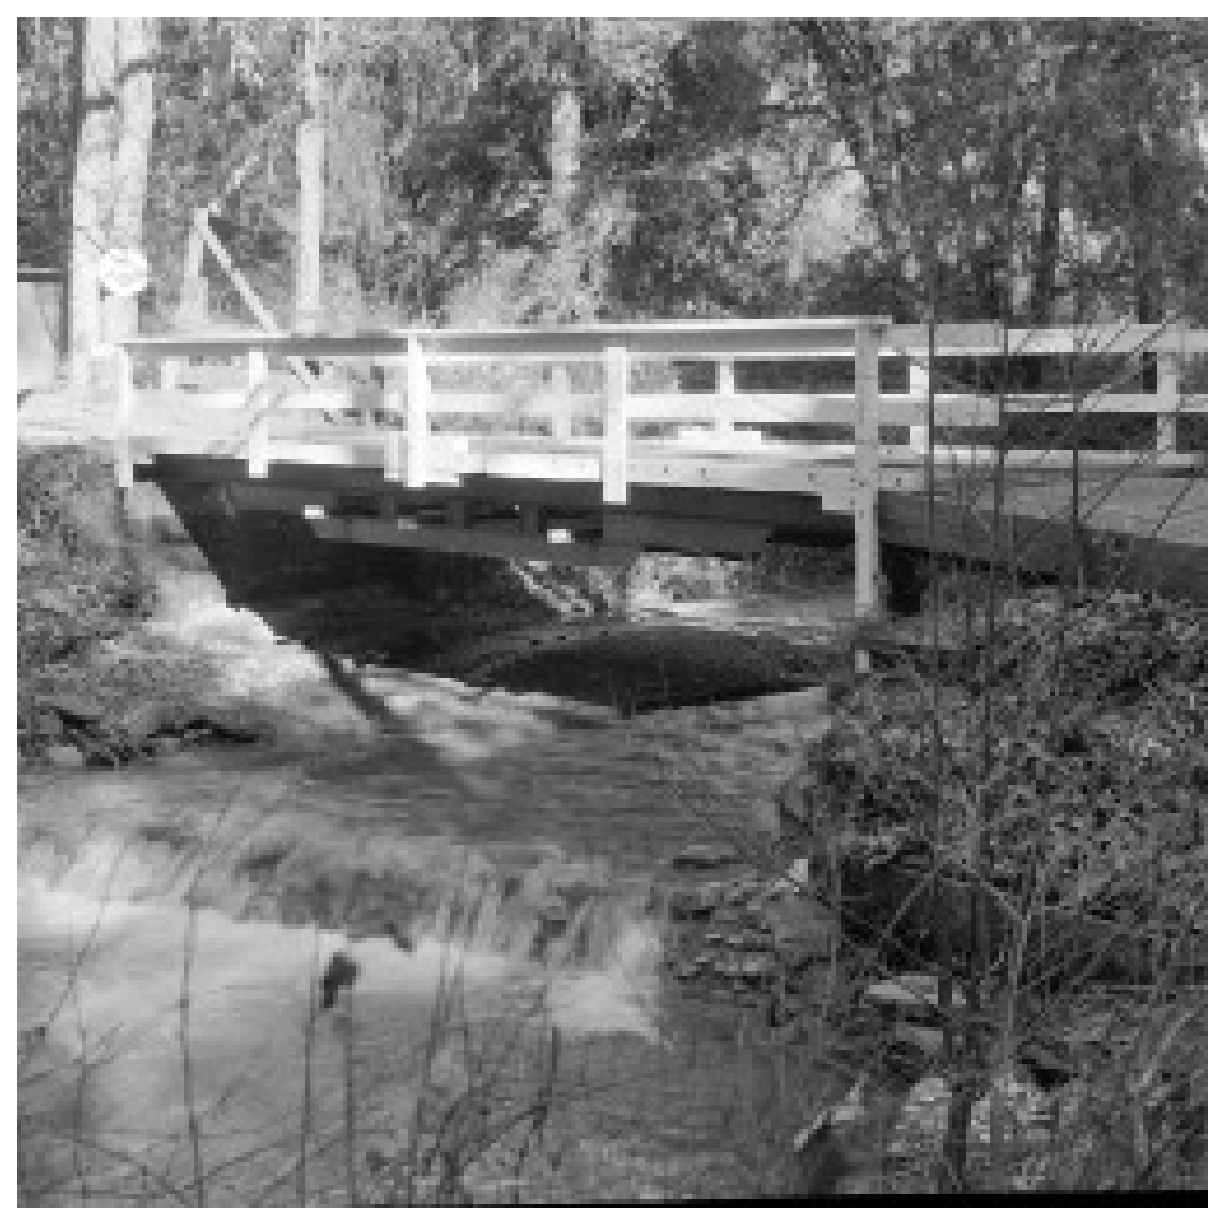
\includegraphics[width=3in]{bridge.eps}
    \caption{The ``Bridge'' image}
    \label{fig:1}
\end{figure}
\end{verbatim}
\begin{figure}[h]
    \centering
    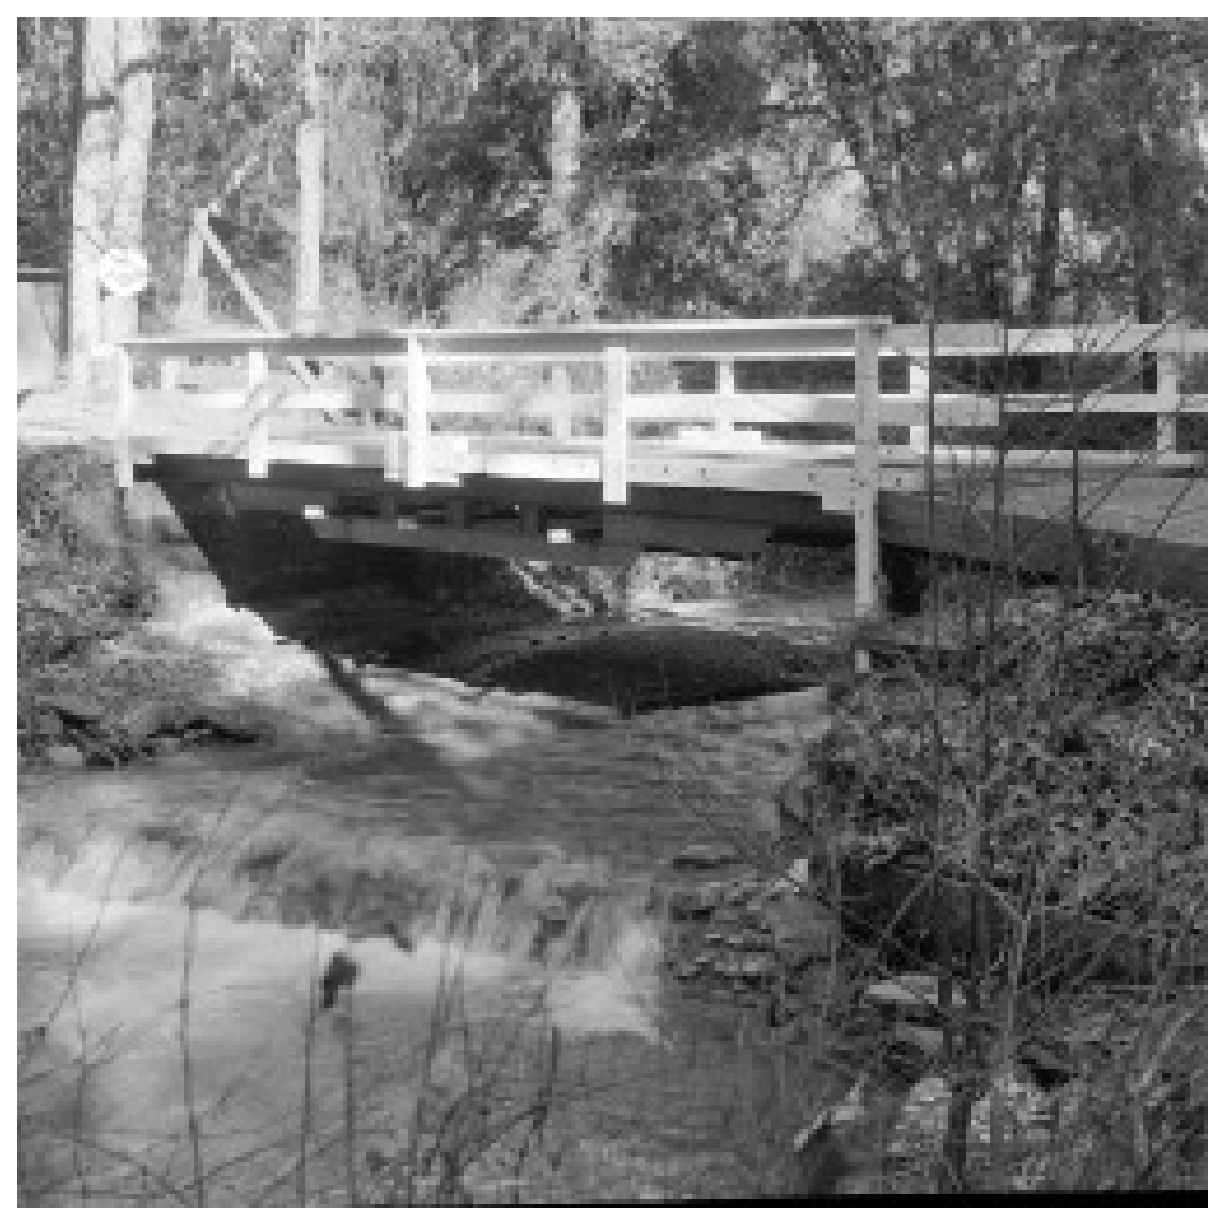
\includegraphics[width=4in]{bridge.eps}
    \caption{The ``Bridge'' image}
    \label{fig:1}
\end{figure}
\texttt{bridge.eps} is a postscript file converted from an image file.
Note that figure \ref{fig:1} is also labeled and cross-referenced here.
For more details about graphics file inclusion, please refer to
\texttt{graphics} package of \LaTeXe.  \LaTeXe\ has a few commands to draw
simple pictures.  Figure \ref{fig:2} shows a picture drawn with \LaTeXe\
commands in the \texttt{picture} environment.  The user can read
\cite{lp:latex} for details.

\begin{figure}
  \centering
\unitlength 0.8in	     % make unit length to be 0.8 inch
\begin{picture}(6,4)(0,0)    % picture coordinates 6 in width, 4 in height,
			     % origin 0,0
\put(1.4,2.6){\line(3,-1){3.0}}   % draw a straight line at slope -1/3
				  % starting at (1.4,2.6) of length 3.0
\put(0,0){\vector(1,0){5.5}}
\put(0,0){\vector(0,1){3}}
\end{picture}

\caption{A Picture Drawn with \LaTeX\ Commands}\label{fig:2}
\end{figure}

\section{Tables-Inserting and Drawing}
Tables and figures are inserted labeled and so on in rather similar ways
except the caption for a table usually appears on top of the table instead
of below that. An example of table is given in Table~\ref{tab:1}. Note
also that this table is written in \textbf{minipage} environment.

\begin{table}
\begin{minipage}[t]{6in}
\caption{Text Formatting and Word Processing Packages}\label{tab:1}
\begin{center}
\begin{tabular}{|l|l|l|}  \hline
	    & Scribe \\ \cline{2-2}
	    & \TeX   \\ \cline{2-2}
Text Formatters\footnote{All the text formatters listed are command-driven}%
	    & \LaTeX \\ \cline{2-2}
	    & troff  \\ \hline
	    & WordStar \\ \cline{2-2}
Word processors \footnote{All the word processors listed are menu-driven}%
	    & Word Perfect  \\ \cline{2-2}
	    & Ms Word	\\ \cline{2-2}
	    & MacWrite	\\ \hline
\end{tabular}
\end{center}
\end{minipage}
\end{table}
Note also that Table~\ref{tab:1} is labeled and referenced. It will be
listed in the LIST OF TABLES.


%%--------------------------------------------------------------------------
\chapter{SPECIAL SYMBOLS}
%%--------------------------------------------------------------------------

\TeX\ has pre-defined many useful special symbols, such as the Greek
letters, mathematical symbols, accented European letters. The newer
version of \TeX\ has even introduced some sets of fonts for some foreign
languages.
For a thesis writer, the most essential knowledge he needs about the
special symbols is Greek letters and mathematical symbols.

\section{Greek Letters}
In \TeX\ and \LaTeXe\ Greek letters are called by  their English names,
e.g., alpha, beta. If the first letter is in capital, then \TeX\ outputs
a capital Greek letter (but many capital Greek letters coincide with
English letters, and hence no commands are designed for them).
The commands for all the Greek letters are listed in
Table \ref{tab:greek}. Note that Greek letters have to be in math mode,
e.g., $\alpha$.

\section{Other Mathematical Symbols}
Beside the Greek letters there are many more math symbols, for example
the Calligraphic letter $\cal F$ which may used for Fourier and
$\cal L$ for Laplace. The user can refer to the \LaTeXe\ Manual\cite{lp:latex}
pp. 41--50 for more information.  Many mathematical
symbols are listed in Appendix \ref{sec:mathsym}.

\section{Accented European Letters}
In the \LaTeXe\ Manual\cite{lp:latex} pp. 38--39, one can find some help as
for how typeset accented European letters.



% master: main
% format: latex

%%--------------------------------------------------------------------------
\begin{appendices}
%%--------------------------------------------------------------------------

%%--------------------------------------------------------------------------
\chapter{FIRST APPENDIX}
%%--------------------------------------------------------------------------

This is the 1st appendix.  Now alphabetic numbering starts for Appedices.
\ifAMS
\begin{equation}
    A=
    \begin{pmatrix}
	a_{11}&a_{12}&\ldots&a_{1n}\\
	a_{21}&a_{22}&\ldots&a_{2n}\\
	\vdots&\vdots&\ddots&\vdots\\
	a_{m1}&a_{m2}&\ldots&a_{mn}
    \end{pmatrix}
\end{equation}
\else
\begin{equation}
    A=
    \left(
    \begin{array}{cccc}
	a_{11}&a_{12}&\ldots&a_{1n}\\
	a_{21}&a_{22}&\ldots&a_{2n}\\
	\vdots&\vdots&\ddots&\vdots\\
	a_{m1}&a_{m2}&\ldots&a_{mn}
    \end{array}
    \right)
\end{equation}
\fi

%%--------------------------------------------------------------------------
\chapter{MATHEMATICAL SYMBOLS}
%%--------------------------------------------------------------------------
\label{sec:mathsym}

Here is the second appendix.  See how equations, figures, and tables in
appendices are numbered.
\ifAMS
\begin{equation}
    A=
    \begin{pmatrix}
	a_{11}&a_{12}&\ldots&a_{1n}\\
	a_{21}&a_{22}&\ldots&a_{2n}\\
	\vdots&\vdots&\ddots&\vdots\\
	a_{m1}&a_{m2}&\ldots&a_{mn}
    \end{pmatrix}
\end{equation}
\else
\begin{equation}
    A=
    \left(
    \begin{array}{cccc}
	a_{11}&a_{12}&\ldots&a_{1n}\\
	a_{21}&a_{22}&\ldots&a_{2n}\\
	\vdots&\vdots&\ddots&\vdots\\
	a_{m1}&a_{m2}&\ldots&a_{mn}
    \end{array}
    \right)
\end{equation}
\fi
%
\begin{eqnarray}
 \left(\int_{-\infty}^\infty e^{-x^2}\,dx\right)^2
 & =& \int_{-\infty}^\infty\int_{-\infty}^\infty
   e^{-(x^2+y^2)}\,dx\,dy \nonumber \\
 & =& \int_0^{2\pi}\int_0^\infty e^{-r^2}r\,dr\,d\theta \nonumber \\
 & =& \int_0^{2\pi}\left(\left. -\frac{e^{-r^2}}{2}
   \right|_{r=0}^{\infty}\,\right)\,d\theta \nonumber \\
 & =& \pi
\end{eqnarray}

otherwise

\begin{eqnarray}
\textstyle\sin18^\circ={\frac{1}{4}}(\sqrt5-1)\\
\ifAMS
x \in \mathbb{R} \\
\fi
k=1.38\times10^{-23}\rm\,J/^\circ K.
\end{eqnarray}

% Math-mode symbol & verbatim
\def\W#1#2{$#1{#2}$ &\ttfamily\string#1\string{#2\string}}
\def\X#1{$#1$ &\ttfamily\string#1}
\def\Y#1{$\big#1$ &\ttfamily\string#1}
\def\Z#1{\ttfamily\string#1}

%
\begin{table}
\caption{Greek Letters}\label{tab:greek}
\vspace{1ex}
\begin{tabular}{*8l}
\X\alpha	&\X\theta	&\X o		&\X\tau 	\\
\X\beta 	&\X\vartheta	&\X\pi		&\X\upsilon	\\
\X\gamma	&\X\iota	&\X\varpi	&\X\phi 	\\
\X\delta	&\X\kappa	&\X\rho 	&\X\varphi	\\
\X\epsilon	&\X\lambda	&\X\varrho	&\X\chi 	\\
\X\varepsilon	&\X\mu		&\X\sigma	&\X\psi 	\\
\X\zeta 	&\X\nu		&\X\varsigma	&\X\omega	\\
\X\eta		&\X\xi						\\
								\\
\X\Gamma	&\X\Lambda	&\X\Sigma	&\X\Psi 	\\
\X\Delta	&\X\Xi		&\X\Upsilon	&\X\Omega	\\
\X\Theta	&\X\Pi		&\X\Phi
\end{tabular}
\end{table}

\begin{table}
\caption{Binary Operation Symbols}\label{tab:bin}
\vspace{1ex}
\begin{tabular}{*8l}
\X\pm		&\X\cap 	&\X\diamond		&\X\oplus     \\
\X\mp		&\X\cup 	&\X\bigtriangleup	&\X\ominus    \\
\X\times	&\X\uplus	&\X\bigtriangledown	&\X\otimes    \\
\X\div		&\X\sqcap	&\X\triangleleft	&\X\oslash    \\
\X\ast		&\X\sqcup	&\X\triangleright	&\X\odot      \\
\X\star 	&\X\vee 	&\X\lhd$^*$		&\X\bigcirc   \\
\X\circ 	&\X\wedge	&\X\rhd$^*$		&\X\dagger    \\
\X\bullet	&\X\setminus	&\X\unlhd$^*$		&\X\ddagger   \\
\X\cdot 	&\X\wr		&\X\unrhd$^*$		&\X\amalg     \\
\X+		&\X-
\end{tabular}

$^*$ Not predefined in \LaTeXe.
     Use one of the packages  \textsf{latexsym}, \textsf{amsfonts} or
     \textsf{amssymb}.

\end{table}


\begin{table}
\caption{Relation Symbols}\label{tab:rel}
\vspace{1ex}
\begin{tabular}{*8l}
\X\leq		&\X\geq 	&\X\equiv	&\X\models	\\
\X\prec 	&\X\succ	&\X\sim 	&\X\perp	\\
\X\preceq	&\X\succeq	&\X\simeq	&\X\mid 	\\
\X\ll		&\X\gg		&\X\asymp	&\X\parallel	\\
\X\subset	&\X\supset	&\X\approx	&\X\bowtie	\\
\X\subseteq	&\X\supseteq	&\X\cong	&\X\Join$^*$	\\
\X\sqsubset$^*$ &\X\sqsupset$^*$&\X\neq 	&\X\smile	\\
\X\sqsubseteq	&\X\sqsupseteq	&\X\doteq	&\X\frown	\\
\X\in		&\X\ni		&\X\propto	&\X=		\\
\X\vdash	&\X\dashv	&\X<		&\X>		\\
\X:
\end{tabular}

$^*$ Not predefined in \LaTeXe.
     Use one of the packages  \textsf{latexsym}, \textsf{amsfonts} or
     \textsf{amssymb}.

\end{table}


\begin{table}
\caption{Punctuation Symbols}\label{tab:punct}
\vspace{1ex}
\begin{tabular}{*{5}{lp{3.2em}}}
\X,	&\X;	&\X\colon	&\X\ldotp	&\X\cdotp
\end{tabular}
\end{table}

\begin{table}
\caption{Arrow Symbols}\label{tab:arrow}
\vspace{1ex}
\begin{tabular}{*6l}
\X\leftarrow		&\X\longleftarrow	&\X\uparrow	\\
\X\Leftarrow		&\X\Longleftarrow	&\X\Uparrow	\\
\X\rightarrow		&\X\longrightarrow	&\X\downarrow	\\
\X\Rightarrow		&\X\Longrightarrow	&\X\Downarrow	\\
\X\leftrightarrow	&\X\longleftrightarrow	&\X\updownarrow \\
\X\Leftrightarrow	&\X\Longleftrightarrow	&\X\Updownarrow \\
\X\mapsto		&\X\longmapsto		&\X\nearrow	\\
\X\hookleftarrow	&\X\hookrightarrow	&\X\searrow	\\
\X\leftharpoonup	&\X\rightharpoonup	&\X\swarrow	\\
\X\leftharpoondown	&\X\rightharpoondown	&\X\nwarrow	\\
\X\rightleftharpoons	&\X\leadsto$^*$
\end{tabular}

$^*$ Not predefined in \LaTeXe.
     Use one of the packages  \textsf{latexsym}, \textsf{amsfonts} or
     \textsf{amssymb}.

\end{table}

\begin{table}
\caption{Miscellaneous Symbols}\label{tab:ord}
\vspace{1ex}
\begin{tabular}{*8l}
\X\ldots	&\X\cdots	&\X\vdots	&\X\ddots	\\
\X\aleph	&\X\prime	&\X\forall	&\X\infty	\\
\X\hbar 	&\X\emptyset	&\X\exists	&\X\Box$^*$	\\
\X\imath	&\X\nabla	&\X\neg 	&\X\Diamond$^*$ \\
\X\jmath	&\X\surd	&\X\flat	&\X\triangle	\\
\X\ell		&\X\top 	&\X\natural	&\X\clubsuit	\\
\X\wp		&\X\bot 	&\X\sharp	&\X\diamondsuit \\
\X\Re		&\X\|		&\X\backslash	&\X\heartsuit	\\
\X\Im		&\X\angle	&\X\partial	&\X\spadesuit	\\
\X\mho$^*$	&\X.		&\X|
\end{tabular}

$^*$ Not predefined in \LaTeXe.
     Use one of the packages  \textsf{latexsym}, \textsf{amsfonts} or
     \textsf{amssymb}.

\end{table}

\begin{table}
\caption{Variable-sized  Symbols}\label{tab:op}
\vspace{1ex}
\begin{tabular}{*6l}
\X\sum		&\X\bigcap	&\X\bigodot	\\
\X\prod 	&\X\bigcup	&\X\bigotimes	\\
\X\coprod	&\X\bigsqcup	&\X\bigoplus	\\
\X\int		&\X\bigvee	&\X\biguplus	\\
\X\oint 	&\X\bigwedge
\end{tabular}
\end{table}


\begin{table}
\caption{Log-like Symbols}\label{tab:log}
\vspace{1ex}
\begin{tabular}{*8l}
\Z\arccos &\Z\cos  &\Z\csc &\Z\exp &
	   \Z\ker    &\Z\limsup &\Z\min &\Z\sinh \\
\Z\arcsin &\Z\cosh &\Z\deg &\Z\gcd &
	   \Z\lg     &\Z\ln	&\Z\Pr	&\Z\sup  \\
\Z\arctan &\Z\cot  &\Z\det &\Z\hom &
	   \Z\lim    &\Z\log	&\Z\sec &\Z\tan  \\
\Z\arg	  &\Z\coth &\Z\dim &\Z\inf &
	   \Z\liminf &\Z\max	&\Z\sin &\Z\tanh
\end{tabular}
\end{table}


\begin{table}
\caption{Delimiters\label{tab:dels}}
\vspace{1ex}
\begin{tabular}{*8l}
\X(		&\X)		&\X\uparrow	&\X\Uparrow	\\
\X[		&\X]		&\X\downarrow	&\X\Downarrow	\\
\X\{		&\X\}		&\X\updownarrow &\X\Updownarrow \\
\X\lfloor	&\X\rfloor	&\X\lceil	&\X\rceil	\\
\X\langle	&\X\rangle	&\X/		&\X\backslash	\\
\X|		&\X\|
\end{tabular}
\end{table}

\begin{table}
\caption{Large Delimiters\label{tab:ldels}}
\vspace{1ex}
\begin{tabular}{*8l}
\Y\rmoustache&	\Y\lmoustache&	\Y\rgroup&	\Y\lgroup\\[5pt]
\Y\arrowvert&	\Y\Arrowvert&	\Y\bracevert
\end{tabular}
\end{table}

\begin{table}
\caption{Math mode accents}\label{tab:accent}
\vspace{1ex}
\begin{tabular}{*{10}l}
\W\hat{a}     &\W\acute{a}  &\W\bar{a}	  &\W\dot{a}	&\W\breve{a}\\
\W\check{a}   &\W\grave{a}  &\W\vec{a}	  &\W\ddot{a}	&\W\tilde{a}\\
\end{tabular}
\end{table}

\begin{table}
\caption{Some other constructions}\label{tab:other}
\vspace{1ex}
\begin{tabular}{*4l}
\W\widetilde{abc}	&\W\widehat{abc}			\\
\W\overleftarrow{abc}	&\W\overrightarrow{abc} 		\\
\W\overline{abc}	&\W\underline{abc}			\\
\W\overbrace{abc}	&\W\underbrace{abc}			\\[5pt]
\W\sqrt{abc}		&$\sqrt[n]{abc}$&\verb|\sqrt[n]{abc}|	\\
$f'$&\verb|f'|          &$\frac{abc}{xyz}$&\verb|\frac{abc}{xyz}|
\end{tabular}
\end{table}


%%--------------------------------------------------------------------------
\chapter{THIRD APPENDIX}
%%--------------------------------------------------------------------------

Here is the third appendix.
Watch the number of Figure \ref{fig:3} in this appendix.

\begin{figure}[h]
  \centering
  \unitlength 1in	    % make unit length to be 1 inch
  \begin{picture}(6,4)(0,0) % picture coordinates 6 in width, 4 in height,
			    % origin 0,0
    \put(1.4,2.6){\line(3,-1){3.0}} % draw a straight line at slope -1/3
				% starting at (1.4,2.6) of length 3.0
    \put(0,0){\vector(1,0){5.5}}
    \put(0,0){\vector(0,1){3}}
  \end{picture}
  \caption{A Picture Drawn with \LaTeX\ Commands}\label{fig:3}
\end{figure}

%%--------------------------------------------------------------------------
\end{appendices}
%%--------------------------------------------------------------------------

	% appendices
%%--------------------------------------------------------------------------

%\nocite{*}
%% \bibliography{ref}
%% \bibliographystyle{ieeetr}

\begin{thebibliography}{99}

\bibitem{lp:latex} \mbox{Leslie Lamport}, \emph{A Document Preparation
 System: \LaTeX\ User's Guide \& Reference Manual}, Published by
Addison-Wesley Publishing Company, 1994.

\bibitem{jbw:tex} \mbox{Jingbai Wang}, \emph{An Introduction to
\TeX/\LaTeX}, the \textbf{on-line documentation} written for CIS,
 University of Pittsburgh, 1988.

\bibitem{pitteng:thesis} \mbox{Engineering Graduate Administrative Committee},
\emph{A Manual for Preparation of Theses and Dissertations
for the School of Engineering}, School of Engineering, University of
Pittsburgh, 1995

\bibitem{pittstd:thesis} \mbox{Kit Ayars}, \emph{Style And Form Manual for
Graduate Thesis and Dissertation Preparation at the University of Pittsburgh},
\verb|http://www.pitt.edu/~graduate/style.html|,
Office of the Provost, University of Pittsburgh, 1995.


\end{thebibliography}

\end{document}		% End of document.
